\label{ch:design}

\section{Bottom-up Abstraction}
\label{sec:bottom-up}
To gain an overview in how the ESL model can be be formed, a complete set of properties is developed bottom-up with the format of generated properties in mind.
When developing the property set for the AHB system, abstraction is a priority. The entire RTL model is therefore ideally verified in a single cluster. 
It is on the other hand not feasible to represent this multi-master design without separating the master agents into their own clusters. The reason for this is 
parallelism and the exponential growth in possible states it brings forth. Every master agent acts with independence between idle and request. This means that the properties must capture all possibilities of each input notify signals and requests in every property, which is not feasible already with two master agents.
\begin{wrapfigure}[14]{l}{8cm}
\includegraphics[width=8cm]{figs/Verif/Verif_block.png}
\caption{Verification clusters}\label{fig:verif-clust}
\end{wrapfigure} 

Fig.~\ref{fig:verif-clust} provides an overview of the verification clusters and their connections. I/O connections are listed with their compound names with port type indicated in the legend. The master agent is a relatively simple design so this section is mainly focused on the matrix cluster. The Gap Free Verification process introduced in Sec.~\ref{sub:gfv} is carried out on the matrix cluster. \par
It is not possible to determine every state of the matrix cluster by observing internal registers alone. There are no registers differentiating between a default master being idle or in the data phase of a transfer. Looking at signal values in the past require constraints on wait states. A better alternative is to define the state of the default master agent as an output to its cluster and an input to the matrix cluster. The states are determined based on this signal, address and data bus ownership as well as slave notify signals. The minimum Conceptual State Machine is listed below, possible transitions are indicated by numbering. 
\begin{enumerate}
 \item Idle: No transfer in progress, \textbf{HREADY} is set and bus is ready to accept a new request (1,2).
 \item Address: A transfer is initiated, \textbf{HREADY} is set and bus is ready to accept a new request.(3)
 \item Slave(x)\_write: Important state for each slave output. (4)
 \item Slave(x)\_read: Important state for each slave input (5)
 \item Data\_end: A transfer is completed, \textbf{HREADY} is set and bus is ready to accept a new request. (1,2,3) 
\end{enumerate}

Operation properties must cover all possible requests, read and write transaction to all slaves, success and error response from slaves as well a transaction to the default slave. Most properties have a duration of one, with write transactions, error response from slave and default slave response as exceptions, which lasts two time points. 

Registers in the arbiter RTL module store the address and data bus ownerships in \textit{master\_sel} and \textit{r\_master\_sel} respectively. The address and data bus signals are multiplexed master agent outputs, with selection based on bus ownership. Because they are not outputs of registers within the design, the values on the bus at time \ITLKW{t}+1 is dependent on the outputs of associated agent at time \ITLKW{t}+1. The generated properties can only reflect values on \textit{X} at time \ITLKW{t}+1 based on values of \textit{Y} at time \ITLKW{t}. ITL offers the \ITLKW{next} operator, which solves this issue. The \ITLKW{next} operator is assigned to the inputs from master agents. \par
The remaining determination requirements are signal outputs. Slave notify signals and \textbf{HREADY} must be determined at all times. Slave outputs need only be determined when their associated notify is set. \textbf{HGRANTx} must be determined whenever \textbf{HREADY} is set, whereas \textbf{HRESP} and \textbf{HRDATA} need only be determined when a slave responds. It is currently not feasible to represent this in the ESL model, so all master agent outputs are determined when \textbf{HREADY} is set. \par
\textbf{HGRANTx} is also not a register output and may change its value before the clock edge, which means a request at time \ITLKW{t} is granted at time \ITLKW{t}. This is the same issue as with the buses, but in opposite time direction. The \ITLKW{prev} operator assigned to \textbf{HGRANTx} can solve this issue. It can altenatively be assigned as the output of a function, which is shown in Sec.~\ref{sec:refine}. \par 
This section has described the essentials for proving completeness on the matrix cluster for single transfers. Extended functionality such as burst transfers are briefly discussed in Sec.~\ref{sec:burst}
 

\section{ESL}
After a complete set of abstract properties for the bus matrix is derived, the ESL model is developed. In the previous section it was established that master agents must be verified in a separate cluster. This translates to the ESL by separating the master agents in their own SystemC-PPA module. Defining a suitable interface between the master agent and bus matrix require careful consideration. \par
With blocking ports, correct simulation behavior and the highest level of abstraction is achieved, but that creates an issue with the bus matrix ESL module for multiple masters. Up to three blocking ports need to be serviced in the same time-point due to parallelism, which is not permitted in SystemC-PPA. A helper module is introduced which is not intended for property generation, but to serve as an emulated port interface. The requirements of this module is described in Sec.~\ref{sub:portem}.

\subsection{Bus matrix}
No more than three explicit states are required to model the bus matrix at the ESL. The communication with the emulated port signals each of these important states in the generated properties. The implementation of the bus matrix ESL covered in Sec.~\ref{sub:bus-matrix} is elaborated with requirements and options. \par
update\_requests->try\_read(\ITLKW{true}, sync, \ITLRW{"state"});  \\
requests\_in->get(reqs); \par

The communication with the emulated port must occur exactly once in all three states. It is what signals the important states 1,2 and 5 from Sec.~\ref{bottom-up}. It is required to be a non-blocking write to unconditionally call a wait, which hands over control to the emulated port before it "gets" the requests. \ITLKW{true} and \textit{sync} offer no function but are required for the function call. \par
Although the arbitration scheme is functionally carried out in the emulated port, it needs to be modeled in the bus matrix to be reflected in the properties. Fixed-priority is chosen in this work, but other arbitration schemes can be modeled by use of a constant function. This is, however, advised against until the functionality can be formally proven within the emulated port itself. Fixed-priority is simple enough to ensure equality by hand. \par
The variables which store the payload of a granted request reflect signals on the address bus, it should therefore not contain \textit{hwdata}. The address bus belongs to the default master if no requests are issued, so its payload gets assigned if that is the case. When the bus transitions $Address\rightarrow Data$, it is distinguished if it is a read or write. In hardware, a write transaction is delayed one cycle to sample data before writing the request to slave. This is modeled by fetching the payload of the appropriate master again, in the case of a write. The correct \textit{hwdata} can be selected by storing address and data bus ownership in variables. A constant function should be used, or property count will increase exponentially with larger configurations. When the transaction is a read, \textit{hwdata} must be zero, otherwise old \textit{hwdata} must be accounted for in each slave. \par
The slave response is broadcast to all master agents, which in this work is carried out through shared ports. The slave response can be forwarded through the emulated port, but with almost no return on investment. It is not done in this work to keep the emulated port minimal. If the slave responds with an error, it is not sufficient to rely on the response payload to relay this information implicitly. Errors must be checked for and if so, assign the error response manually so that a separate property is generated which can be refined to model the two cycle error response. The default slave response, which occur when no slave is selected, is modeled by assigning error status and zero data to all masters.\par
The functionality of \textit{hready} and \textit{hgrant} is carried out in the emulated port, but is only sufficient to represent \textit{hready} in the determination requirements of the completeness description. Separate ports are required to represent \textit{hgrantx} in the determination requirements, although this representation serves no function in simulation. It is possible to represent each \textit{hgrantx} with boolean values, but not without unnecessary overhead. All \textit{hgrantx} must be set/reset for each possibility of requests, which leads to $3*(x+x^2)$ extra lines of code, where x is number of masters. This can be compressed in a constant function, but that leads to increased property proof time. This is unnecessary overhead, as this port serves no function in the model other than I/O coverage in the property set. Therefore it is represented with an enum in this work, which is refined as a function in the properties. \par
\WKSAY{should i talk about state transitions here or is the FSM in implementation enough} 
 

\subsection{Master Agent}
The SystemC-PPA module of the master agent needs to cover all signals of the master agent interface. Some of these signals are represented in the event handling of the blocking ports. \par
mAgent\_request->write(\ITLKW{true}); \par
Models the bus request through the event notify of the port, \ITLKW{true} is just to satisfy the function call. \par
bus\_ready->write(\ITLKW{true}); \par
Models the \textit{hready} signal from the bus through its wait(event) of the port, and is called in the address and data phase of a transfer. The remaining interface values must be written to shared ports and not over this interface. If the agent were to transmit \textit{hwdata} over this port, it will not be read until the data phase is over. Therefore, all remaining interface signals are transmitted though shared ports at the appropriate times according to protocol, before the blocking write occurs.  
 
\subsection{Emulated port}
\label{sub:portem}
The emulated port has strict requirements to ensure correct simulation behavior, both in terms of synchronization and in terms of arbitration. This module can not be proven formally to be a sound abstraction of the RTL for the same reason that it is implemented. The chosen arbitration scheme must be manually verified to exactly match the arbitration scheme in the bus matrix. \par
The port must wait for a synchronization signal from the bus matrix, perform request forwarding, service all applicable blocking ports and return to wait for a synchronization signal without interruption. This is accomplished by utilizing blocking inputs for both ports from each master agent, and performing a non-blocking read, only if there is a writer waiting. 

\begin{C++}
//begin while
update_requests->read(); 
//requests must be reset 
if(mAgent_request->peek()){
mAgent_request->try_read();
requests.mx_request = true;
}
requests_out->set(requests); 
if(bus_ready->peek()) bus_ready->try_read();
//end while
\end{C++}


\section{Refining the Properties}
\label{sec:refine}
This section describes how the generated property sets are refined to hold on the design. Every I/O signal, visible register and important state is represented with a macro, which is of the form \par  
\ITLKW{macro} signal\_name : \ITLIW{type} := refinement \ITLKW{end macro}; \par
Every blocking port in the SystemC-PPA has signal macros for the payload, as well as a set of macros, sync and notify, which represent the wait(event) and event notify respectively. Before covering the individual clusters property refinement, the emulated port interfaces will be explained collectively. \par
The emulated port interfaces exclusively use the sync and notify to convey information. Some of these do not exist in the RTL design, so they are given abstract values to satisfy the properties. Following is a pseudo refinement of the existing signals, with a two master system as example. \par
\ITLKW{macro} agent0\_request\_notify : \ITLIW{boolean} := hbusreq0 \ITLKW{end macro}; \\
\ITLKW{macro} update\_requests\_sync : \ITLIW{boolean} := hbusreq0 \ITLRW{or} hbusreq1 \ITLKW{end macro}; \par
\ITLKW{macro} agent0\_request\_sync : \ITLIW{boolean} := hgrant0 \ITLRW{and} hready0 \ITLKW{end macro}; \\
\ITLKW{macro} agent0\_ready\_sync : \ITLIW{boolean} := hready0 \ITLKW{end macro}; \\
\ITLKW{macro} update\_requests\_notify : \ITLIW{boolean} := \\ hready0 \ITLRW{and} hready1 \ITLRW{or} \ITLCOMMENT{example with two masters} \\  
hgrant0 \ITLRW{and} hready0 \ITLRW{or} \\ hgrant1 \ITLRW{and} hready1 \\ \ITLKW{end macro}; \par
This covers the complete top-level connection of all the signals, as long as this behavior is guaranteed within the emulated port it should not leave a gap in verification. However, this representation is not sufficient to use in the completeness description to determine \textit{hbusreqx} as input, or \textit{hgrantx} as output. The macros generated from the shared interfaces are used in the completeness description for these two signals in addition. The emulated port interface result in a high number of vacuous properties, up to 45\% \par

\subsection{Bus Matrix}

All remaining I/O signals are refined with the similarly named top-level signal. The exceptions are hwrite and hsize and hgrant, which are represented at the ESL using enum values. The first two are conditionally refined with the top-level signals as follows.\\   
\ITLKW{macro} agent0\_sig\_hwrite : \ITLIW{mask} := \ITLKW{if}(\ITLKW{next}agent0.hwrite = \ITLRW{"000"}) \ITLKW{then} MT\_B ...\\
All input signals from master agent which are fetched from shared ports are assigned the \ITLKW{next} operator. \par 
The refinement of hgrant require an added macro which serves as a function to determine its value at any given time. The \ITLIW{type} of hgrant is redefined from mx\_grant to \ITLIW{boolean}. The default master is granted when no other master holds a grant. Every master which is not default master is refined as follows: \\
\ITLKW{if}(hready \ITLRW{and} hbusreqx \ITLRW{and} \ITLRW{not(}higher\_request\ITLRW{)}) \ITLKW{then true}\\
\ITLKW{elsif}(addr\_own = x \ITLRW{and not(}hready\ITLKW{)}) \ITLKW{then true \\else false}  \par
The only visible registers extracted from the ESL model are the address and control signals, address bus ownership and state variables. The data bus variable is optimized away from the SystemC-PPA by DeSCAM, which is not ideal as we need this register to determine the states. A macro for the data bus ownership and the default master state is added to the description. The address and control signals are refined with the address mux outputs in the arbiter module: \\
\ITLKW{macro} AS\_regs\_(xx) : matrix/ahb\_arb0/mst\_in\_sel.(xx) \ITLKW{end macro}; \par
The visible registers extracted from the state variable of the ESL model, are not represented anywhere in the RTL. There are no state variable called phases so an unused type "\textit{phases}" is added to the RTL so that these visible registers can be mapped. \par
The state macros representing the state of communication with slaves are simply refined with their associated notify signal. The remaining states are refined as follows: 
\begin{itemize}
 \item Idle: If default master is not in the state Address or Data, but still owns both address and data bus, the bus is idle.
 \item Address: If default master owns the data bus, but is not in the data phase, and the default master is in the address phase or does not own the address bus, the bus is in state Address. 
 \item Data\_end: update\_requests\_notify is set, default master is in the data phase or does not own the data bus.  
\end{itemize}

Finally, all properties which end with an error signal or starts with a write request on the address bus must be refined so \ITLKW{t\_end}=\ITLKW{t}+2.

\subsubsection{Completeness Description}
All inputs, as well as the default master state are listed with their signal macro names as determination assumptions. \par
All outputs are listed as determination requirements, most of them conditionally. The unconditional signals are the following: \\
\begin{itemize}
 \item \textit{update\_requests\_notify}: determine all \textit{hready}. An assertion which proves that they always have the same value is added as dependency.
 \item \textit{bus\_to\_slave(x)\_notify}
 \item \textit{slave\_to\_bus(x)\_notify} 
\end{itemize}

The top two signals are used as conditions to determine the remaining outputs. The slave outputs are determined if \textit{bus\_to\_slave(x)\_notify} is set and response data payload signals and \textit{hgrantx} are determined if \textit{update\_requests\_notify} is set. \par

The visible registers for the address bus and address bus ownership are listed as local determination requirements. The data bus ownership is not listed here, because it is optimized away from the property set. It is not used to directly determine any outputs so it can be left out without failing any determination checks, although it would ideally be covered by the property set as an added precaution. \par
Finally, in the case of a single master system, an assertion is added to prove that requests can only occur if the master agent is in the corresponding state. This assertion is added to the dependencies of the completeness description so that the case split test holds. 

\subsection{Master Agent}
The property set and completeness description is identical for all master agents, therefore it is only refined for one master. 
All I/O signals except the emulated port interfaces are refined with their similarly named top-level RTL signal. In the master agent, \textit{hsize} is an output, so therefore determining the \ITLKW{if}\ITLRW{(}mAgent\_to\_bus.hsize = \ITLRW{"000"} then MT\_B ... requires an assertion added to the completeness description, which proves this correspondence. \par
The registers storing the requests are refined to mAgent0/(xx)\_reg. \par
All states are refined to the corresponding state of the RTL design.

\section{RTL}
The open source architecture used in this work is defined in one architectural module, in the file \textit{ahb\_arbiter.vhd}. It uses arbitration functions from the file \textit{ahb\_func.vhd}, slave address configurations from \textit{ahb\_configure.vhdl}, packages from \textit{ahb\_package.vhd} and components from \textit{ahb\_component.vhdl}. \par
All payloads visible from the top-level in the ESL design are added to the package file, together with state machine declarations for the master and slave agent, as well as the unused type representing the ESL states of the bus matrix. It also contains some constants to offer readability for the signals which are hardwired. \par
Component declaration of all system modules are added to the component file, this includes agents, arbiter and bus matrix. The bus matrix is a top-level module for the arbiter, which instantiates the arbiter and provides default master selection and master priority. Master zero is highest priority, which decreases with incrementing numbers. For simplicity, the highest priority master is set as the default in this work. \par
The configuration file contains the slave address ranges in decimal number, as well as the remapped address ranges of the slaves. Remap is not implemented in this work so they must be equal, remap is hardwired to zero for extra security. \par
The top-level module must include the following: \par
\ITLKW{library} \ITLIW{ieee}; \\
\ITLKW{use} \ITLIW{ieee}.\ITLIW{logic\_1164}.\ITLKW{all}; \\ 
\ITLKW{use} \ITLIW{ieee}.\ITLIW{numeric\_std}.\ITLKW{all}; \\
\ITLKW{use} \ITLIW{work}.ahb\_package.\ITLKW{all}; \\
\ITLKW{use} \ITLIW{work}.ahb\_components.\ITLKW{all}; \par
The arbiters reset is active low, so the top-level reset must be inverted before assigning it to the matrix port map. All slave agents require their address offset as a generic in the form of a 32-bit logic vector. All master and slave agents are connected to their inputs and outputs of the matrix with corresponding numbers. 

\subsection{Slave Agent}
The slave agent includes the same packages as the top-level, except for the components. It includes an additional package \ITLIW{ieee}.\ITLIW{std\_logic\_unsigned}.\ITLKW{all} so that the slave address offset can be subtracted from the haddr input. \par
It is important that all output signals are register outputs, where hready is an exception, this should be controlled as a combinational output: \\
hready <= '1' \ITLKW{when} section = idle \ITLKW{else} '0'; \par
The module has a state machine comprised of combinational logic, which uses flags to signal when address/control and data gets clocked in. If the transaction is a read, it must zero the \textit{hwdata} output to avoid writing an old data value to the slave. The slave ignores \textit{hwdata} in read transactions, but the property checker does not. \par 
When the response payload is written to the outputs, a flag is set. This flag is used together with \textit{hready} to signal when the default values are assigned to the outputs.

\subsection{Master Agent}
The master agent also implements the state machine in combinational logic. Flags are used to signal when the payload is written to registers and when these registers are written to the bus. It is not currently required to update \textit{hbusreqx} and \textit{htrans} with combinational logic, but this simplifies an extension to burst transfers. The master will fetch a response payload from the master agent regardless of the transaction direction. This is to notify the master on transfer success. This can be configured in the RTL and ESL with little effort, as no modification to the bus matrix is required.  
 

\section{Building the Generator}
The generator consists of two parts; the hardware generator and the plugin which generates and refines the property sets. The hardware generator takes number of masters and slaves as input arguments and reads a text file of slave address ranges which are stored in a map. The generator instantiates two classes with this data which generate the system at the RTL and ESL. The generator produces a text file with the same stored data, converted for use within the plugin. It continues to call the plugin with the bus matrix and master agent SystemC-PPAs in turn. The plugin reads the text file and distinguishes between the two SystemC-PPAs to generate a refined property set and completeness description for each. 

\subsection{Hardware generator}
The generator uses the slave input argument to decide how many lines of the address map text file to read. It recognizes the words "start" and "end" to determine the start and end of the range. A separate map is produced for the ESL and RTL generation to avoid the need to convert the address format on the fly. The classes which generate the ESL and RTL are so similar in structure and function that they will not be described separately. \par
A set of files are generated for each abstraction layer, which are files that are not static with respect to number of masters and slaves. All files such as agents, dummies for test bench and arbiter remain in the output folder untouched and must not be deleted or modified. \par
All files are generated with an output file stream which is assigned a function output. Each file has its own dedicated function which write the module description to a local string stream. Each function uses the stored number of masters, slaves and address map to produce its module according to the requested configuration. 

\subsection{Plugin: PrintAHB}
The plugin starts by reading the plugin data text file, which contain number of masters and slaves, as well as slave address ranges. The slave address ranges were used in an earlier implementation, but are not removed from the plugin data in case they are needed in the future. The plugin checks the file name if it is the bus matrix or master agent and calls the appropriate function to generate the property files. \par
DeSCAM creates an abstract model of the SystemC-PPA which is stored in a C++ object. This object contains maps and objects which together store all I/O signals, all variables, the FSM, property-suite etc. The plugin iterates over the components of the abstract model to simultaneously generate and refine the property macros as well as property set and completeness description.

\subsubsection{Bus matrix}
The I/O signals of the ESL design and RTL are given the same names, which simplify the automatic property refinement. The plugin iterates over a port map, converts the abstract signal name to its corresponding RTL signal name and writes it to a string stream. Some signals require more elaborate refinements, as is covered in Sec.~\ref{sec:refine}. These signals are checked for with if-else statements and refined accordingly when found. \par
The required assertions and macro functions are added for the appropriate number of masters, based on data from the input text file. The macros for data bus ownership and default master state are subsequently added. The visible registers do not share signal names with the RTL design, so every one is checked for by name and refined accordingly. \par
The states are given recognizable names and numbering in the ESL model, which are transferred to the abstract model but with added numbering. The plugin iterates over the state map and refines the state macro according to name. If the state contains important numbering, this number is fetched with a function that excludes the numbering added by the tool. \par
Each operation property is generated using functions which are slightly modified versions of functions from the plugin \textit{PrintITL} from \cite{descam}. Mainly, it modifies the time-points in the properties which require two cycles to complete by checking the assumptions and commitments. A property is only generated if it is not vacuous by checking if there is a conflict in the assumptions related to the emulated port interface. Some of these conflicts lead to conflicts in the completeness check and must be removed. Finally, the number of non-vacuous and vacuous properties are printed to the terminal.\par

\subsubsection{Master agent}
The master agent is refined to hold on master agent zero in a similar, but simpler manner than the bus matrix. There are no vacuous properties which need to be removed. 



\section{Simulation}
\label{sec:sim}


\section{Experimental Results}
Comparisons are made between the RTL model and its PPA representation, to determine the efficacy of the abstraction. Table \ref{tab:stats} compare the resource demand of the different models with respect to configuration size. The variables lister in the PPA section are variables available in the abstract model and does not count intermediate variables used in the ESL model. One additional input and visible register are added to the property set during the refinement process, which are are also not listed in the table. The listings for the bus matrix are the sum of all three rows.

\begin{table}[hbt] 
  \begin{tabular}{ l r r r r r}
  \hline 
  \hline
      & \multicolumn{2}{c}{\textbf{\_\_\_}RTL\textbf{\_\_\_}} & \multicolumn{3}{c}{\textbf{\_\_\_\_\_\_}PPA\textbf{\_\_\_\_\_\_}} \\
  Modules & inp./out. & FFs & inp./out & var. & states \\
    \hline
  Master agent & 107/114 & 175 & 2/4 & 12 & 5 \\
  \hline
  Bus matrix & - & 114 & 1/1 & 5 & 3 \\
  
  Per slave & 107/114 & 193 & 1/1 & - & 2 \\
 
  Per master & 106/47 & 111 & 1/1 & - & - \\
    \hline
    \hline  
  \end{tabular}
\caption{AHB resource comparison}
\label{tab:stats}
\end{table}

The simulation models introduced in Sec.~\ref{sec:sim} were run on a range of configurations. The efficiency of simulating at the ESL compared to the RTL is clear. The simulations ran for a total of $10^6$ transactions, independent of configuration size, where the ESL simulation time was 7-8 seconds in all cases, with the variation occurring for different runs on the same configuration. The RTL simulation times are shown in the figure below. All simulations were run on the same computer on the same day. The ESL models were built and run with cmake3, whereas the RTL models were built and run with Modelsim SE-64 10.7c. All RTL simulations were run without displaying signals as waveforms. \\
\WKSAY{These simulations are run locally at uni because frascati was to variable and kept disconnecting. What is interesting is that while ESL simulation ran at 6-7 seconds, the RTL simulations ran much slower than shown here, with almost a minute in difference in some cases}

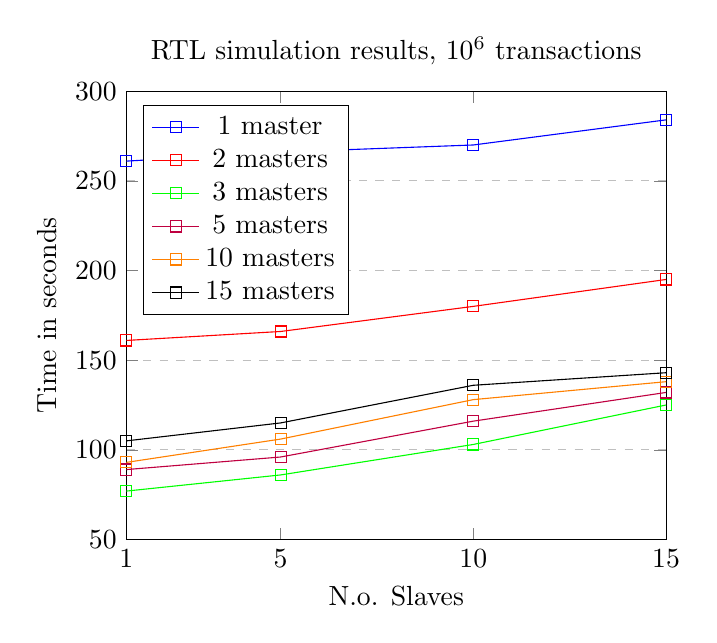
\begin{tikzpicture}
\begin{axis}[
    title={RTL simulation results, $10^6$ transactions},
    xlabel={N.o. Slaves},
    ylabel={Time in seconds},
    xmin=1, xmax=15,
    ymin=50, ymax=300,
    xtick={1,5,10,15},
    ytick={50,100,150,200,250,300},
    legend pos=north west,
    ymajorgrids=true,
    grid style=dashed,
]
\addplot[
    color=blue,
    mark=square,
    ]
    coordinates {
    (1,261)(5,266)(10,270)(15,284)

    };
    \addlegendentry{1 master}

\addplot[
    color=red,
    mark=square,
    ]
    coordinates {
    (1,161)(5,166)(10,180)(15,195)
    };
    \addlegendentry{2 masters}

\addplot[
    color=green,
    mark=square,
    ]
    coordinates {
    (1,77)(5,86)(10,103)(15,125)
    };
    \addlegendentry{3 masters}

\addplot[
    color=purple,
    mark=square,
    ]
    coordinates {
   (1,89)(5,96)(10,116)(15,132)
    };
    \addlegendentry{5 masters}

\addplot[
    color=orange,
    mark=square,
    ]
    coordinates {
    (1,93)(5,106)(10,128)(15,138)
    };
    \addlegendentry{10 masters}

\addplot[
    color=black,
    mark=square,
    ]
    coordinates {
    (1,105)(5,115)(10,136)(15,143)
    };
    \addlegendentry{15 masters}
    
\end{axis}
\end{tikzpicture}

The simulation time of configurations with one and two masters are offset due to the delay between transfers. The simulations are therefore not slower for configurations with one and two masters, they merely need more cycles to complete the $10^6$ transfers
This latency is induced by the blocking interface between the agent and master, with the payload response for write transactions added on top. \par

The amount of generated properties depend on amount of masters and slaves connected to the system. The figure below show the relationship between properties and configuration sizes. Vacuous properties are not counted. The proof time of each properties varies between 1-10 seconds for the small configurations up to 1-2 minutes for the largest.

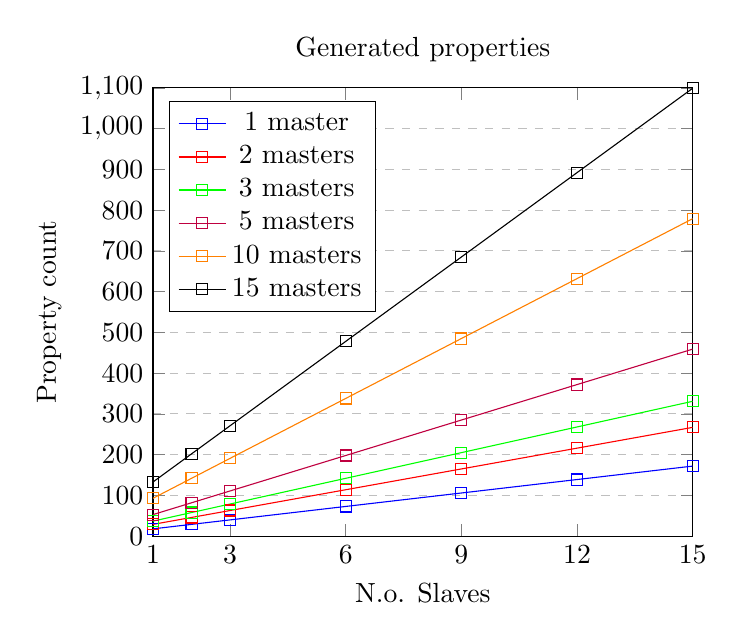
\begin{tikzpicture}
\begin{axis}[
    title={Generated properties},
    xlabel={N.o. Slaves},
    ylabel={Property count},
    xmin=1, xmax=15,
    ymin=0, ymax=1100,
    xtick={1,3,6,9,12,15},
    ytick={0,100,200,300,400,500,600,700, 800, 900, 1000, 1100},
    legend pos=north west,
    ymajorgrids=true,
    grid style=dashed,
]
\addplot[
    color=blue,
    mark=square,
    ]
    coordinates {
    (1,18)(2,29)(3,40)(6,73)(9,106)(12,139)(15,172)

    };
    \addlegendentry{1 master}

\addplot[
    color=red,
    mark=square,
    ]
    coordinates {
    (1,29)(2,46)(3,63)(6,114)(9,165)(12,216)(15,267)
    };
    \addlegendentry{2 masters}

\addplot[
    color=green,
    mark=square,
    ]
    coordinates {
    (1,37)(2,58)(3,79)(6,142)(9,205)(12,268)(15,331)
    };
    \addlegendentry{3 masters}

\addplot[
    color=purple,
    mark=square,
    ]
    coordinates {
   (1,53)(2,82)(3,111)(6,198)(9,285)(12,372)(15,459)
    };
    \addlegendentry{5 masters}

\addplot[
    color=orange,
    mark=square,
    ]
    coordinates {
    (1,93)(2,142)(3,191)(6,338)(9,485)(12,632)(15,779)
    };
    \addlegendentry{10 masters}

\addplot[
    color=black,
    mark=square,
    ]
    coordinates {
    (1,133)(2,202)(3,271)(6,478)(9,685)(12,892)(15,1099)
    };
    \addlegendentry{15 masters}
    
\end{axis}
\end{tikzpicture}




\section{Concept: Burst Transfers}
\label{sec:burst}
